\section{Methods}



\subsection{Aggregation}
We will use Manuele Brambilla's \cite{Brambilla2013} taxonomy of collective swarm behaviors, in Figure \ref{fig:taxonomy}, to show the context for the modeled aggregation behavior. Behaviors categorized as spatially-organizing distribute robots and objects in space. These behaviors serve as fundamental building blocks for more advanced swarm behaviors, as they enable robots to connect, communicate, and interact with one another. Aggregation, the simplest of collective behaviors, groups all robots of a swarm in a region of the environment. If we assume that the robots' environment is unbounded we will have two design choices. The aggregation algorithm will either have to allow a robot to reconnect with the group or never let it disconnect from it. The first approach involves access to external information about the position of the swarm e.g. robot coordinates. The second approach relies on robots being initially connected.

% Taxonomy
\begin{figure}[H]
\caption{Taxonomy of collective swarm behaviours \cite{Brambilla2013}}
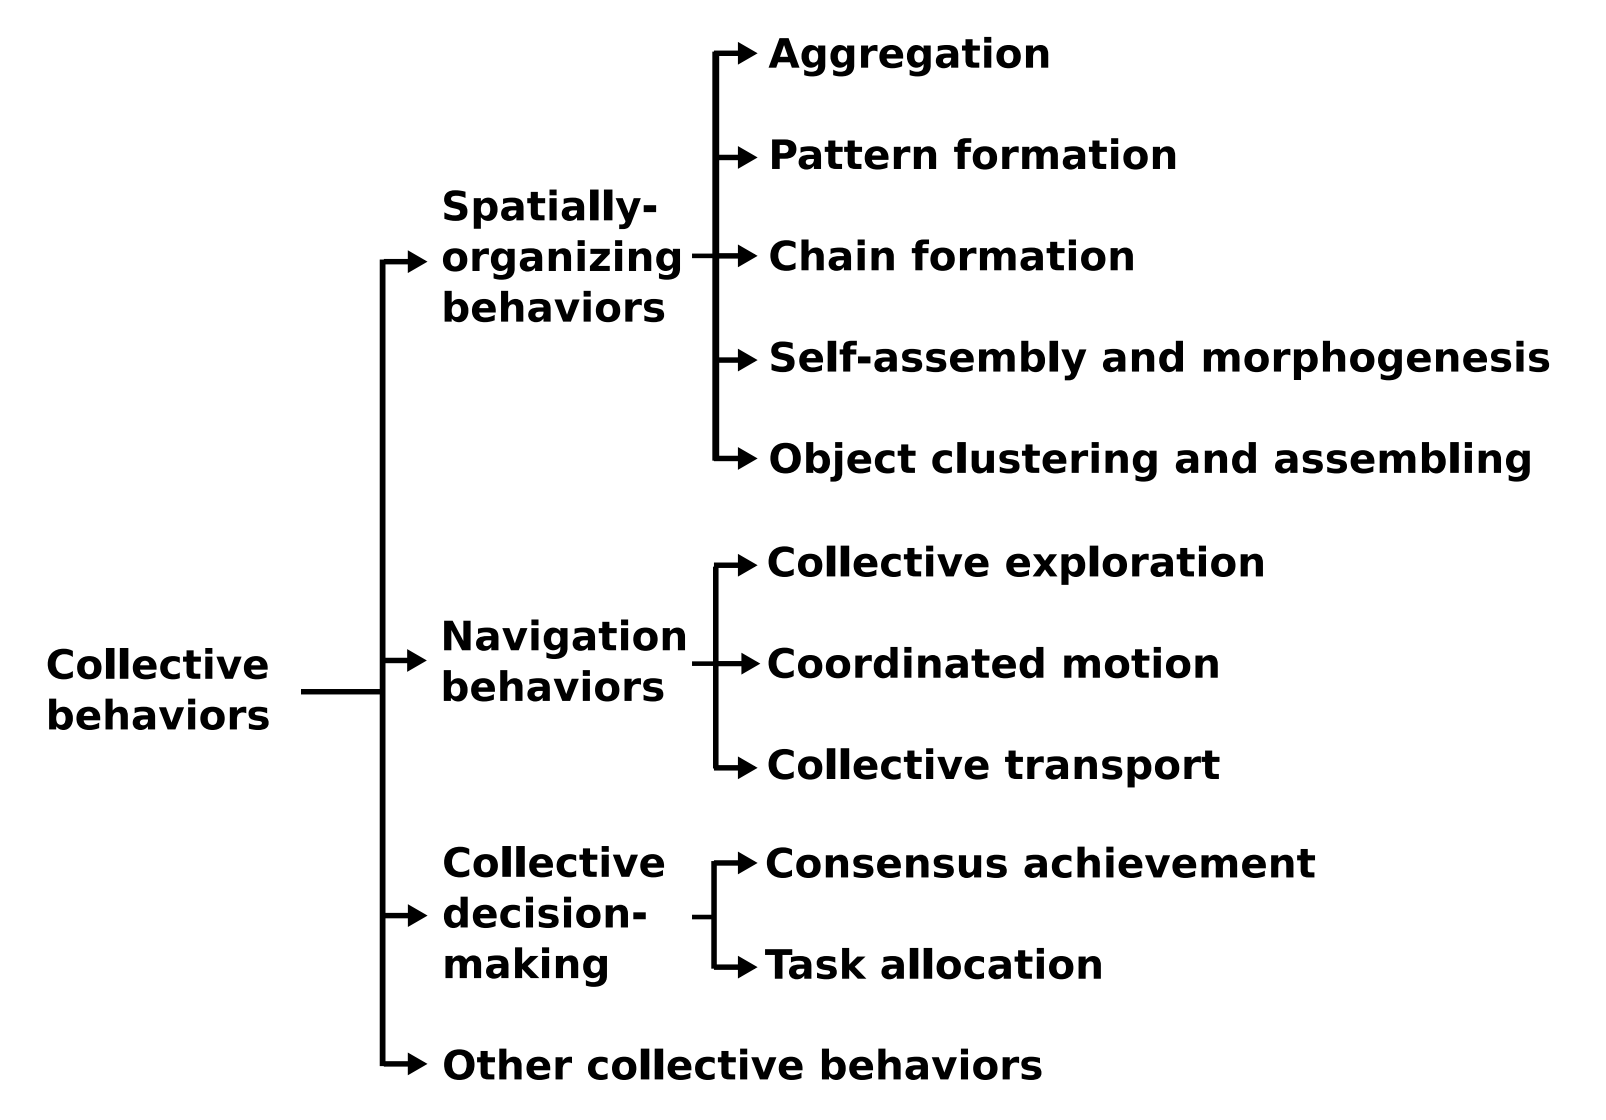
\includegraphics[width=\textwidth]{images/taxonomy.png}
\label{fig:taxonomy}
\end{figure}



\subsection{Beta Algorithm}

% Pseudo-code for Beta algorithm
\begin{figure}[H]
\caption{Pseudo-code for Beta algorithm \cite{Nembrini2002}}
\begin{lstlisting}[style=code]
Create list of neighbours for robot, Nlist
k = number of neighbours in Nlist
i = 0

loop forever {
	i = i modulo cadence

	if (i = 0) {
		Send ID message

		Save copy of k in LastK
		Set reaction indicator Back to FALSE
		k = number of neighbours in Nlist
		Create LostList comparing Nlist and OldList

		for (each robot in LostList) {
			Find nShared, number of shared neighbours
			if (nShared <= beta) {
				Set reaction indicator Back to TRUE
			}
		}

		if (Back = TRUE) {
			turn robot through 180 degrees
		}
		else if (k > LastK) {
			make random turn
		}
		
		Save copy of Nlist in Oldlist
	}
	Steer the robot according to state
	Listen for calls from robots in range
	Grow Nlist with neighbours IDs and connection info

	i++
}
\end{lstlisting}
\label{fig:pseudocode}
\end{figure}


\subsection{Movement}



\subsection{Connection}



\subsection{System variables}



\subsection{Automaton}

% Automaton
\begin{figure}[H]
\caption{Timed automaton for the Beta algorithm}
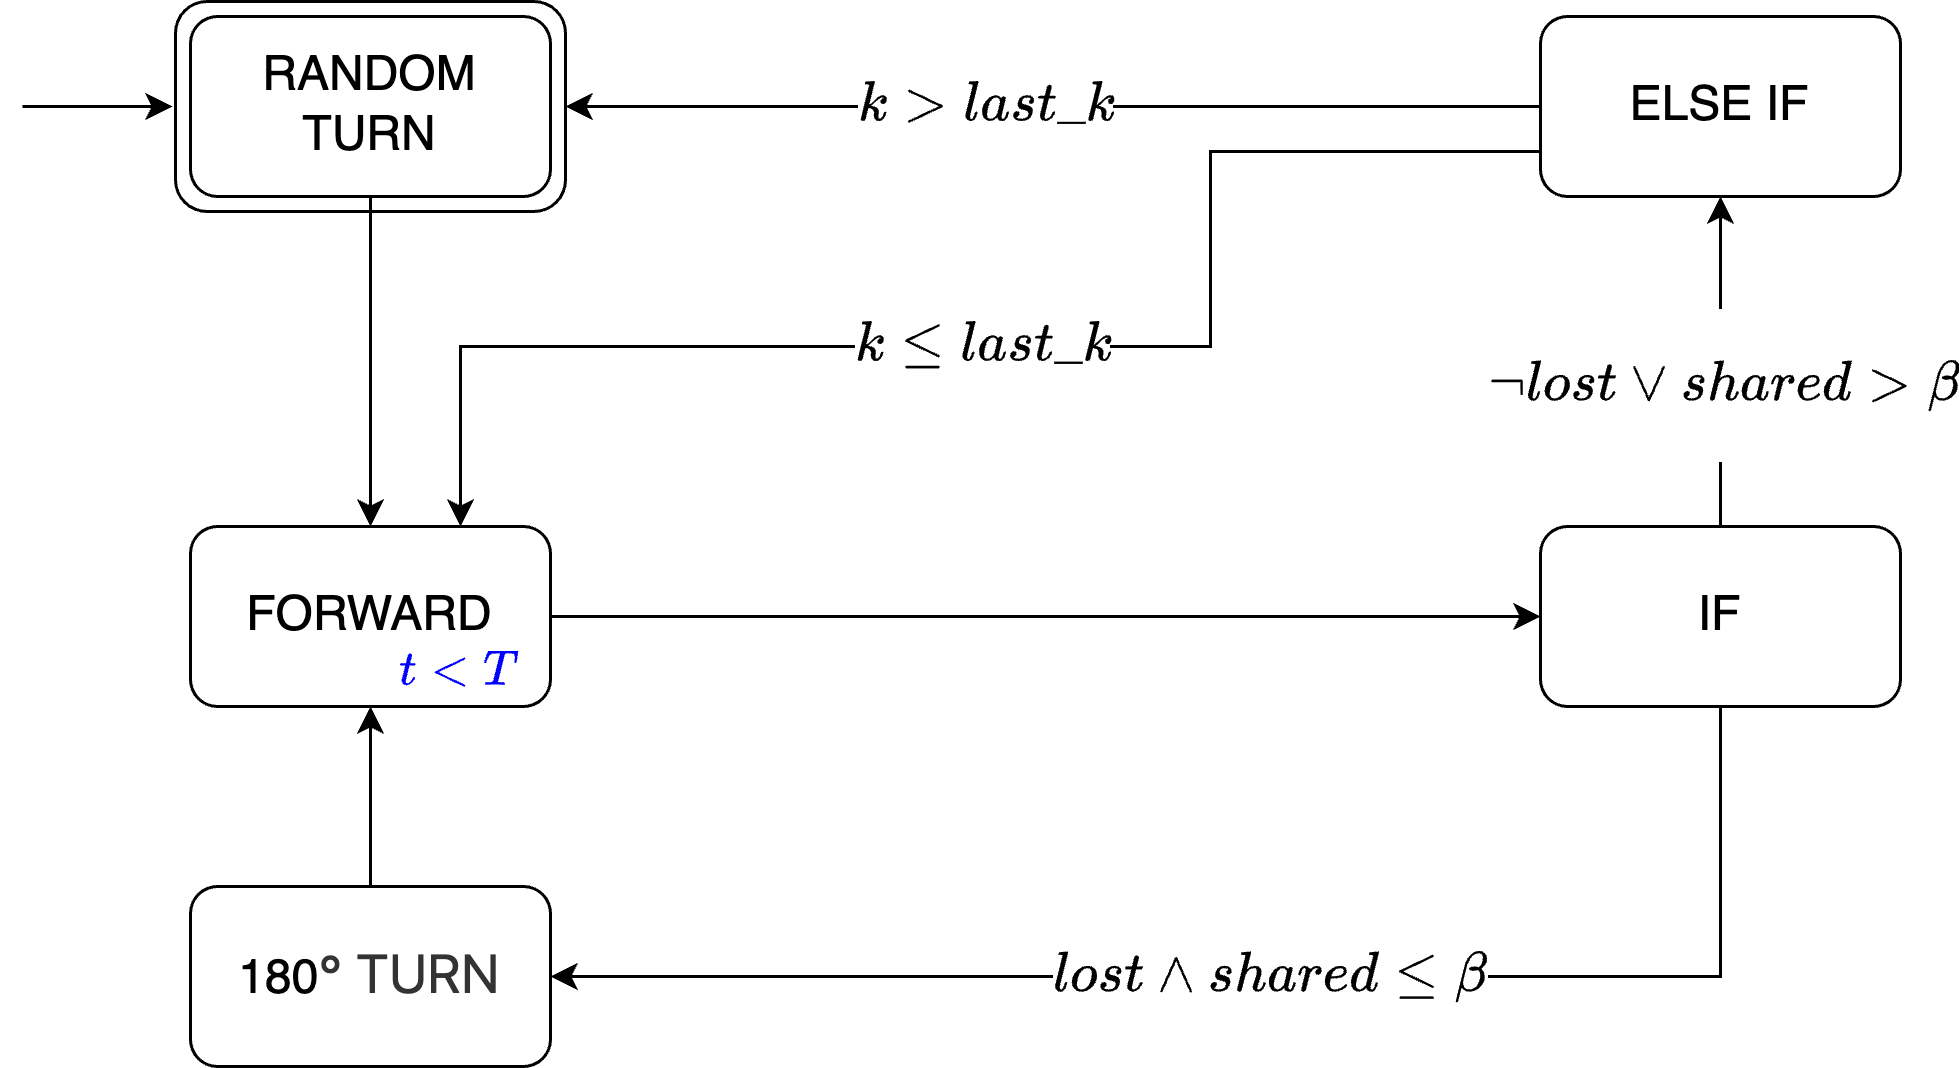
\includegraphics[width=\textwidth]{images/beta.png}
\label{fig:automaton}
\end{figure}
